\section*{Math 202A - HW8 - Dan Davison - \texttt{ddavison@berkeley.edu}}
\begin{mdframed}
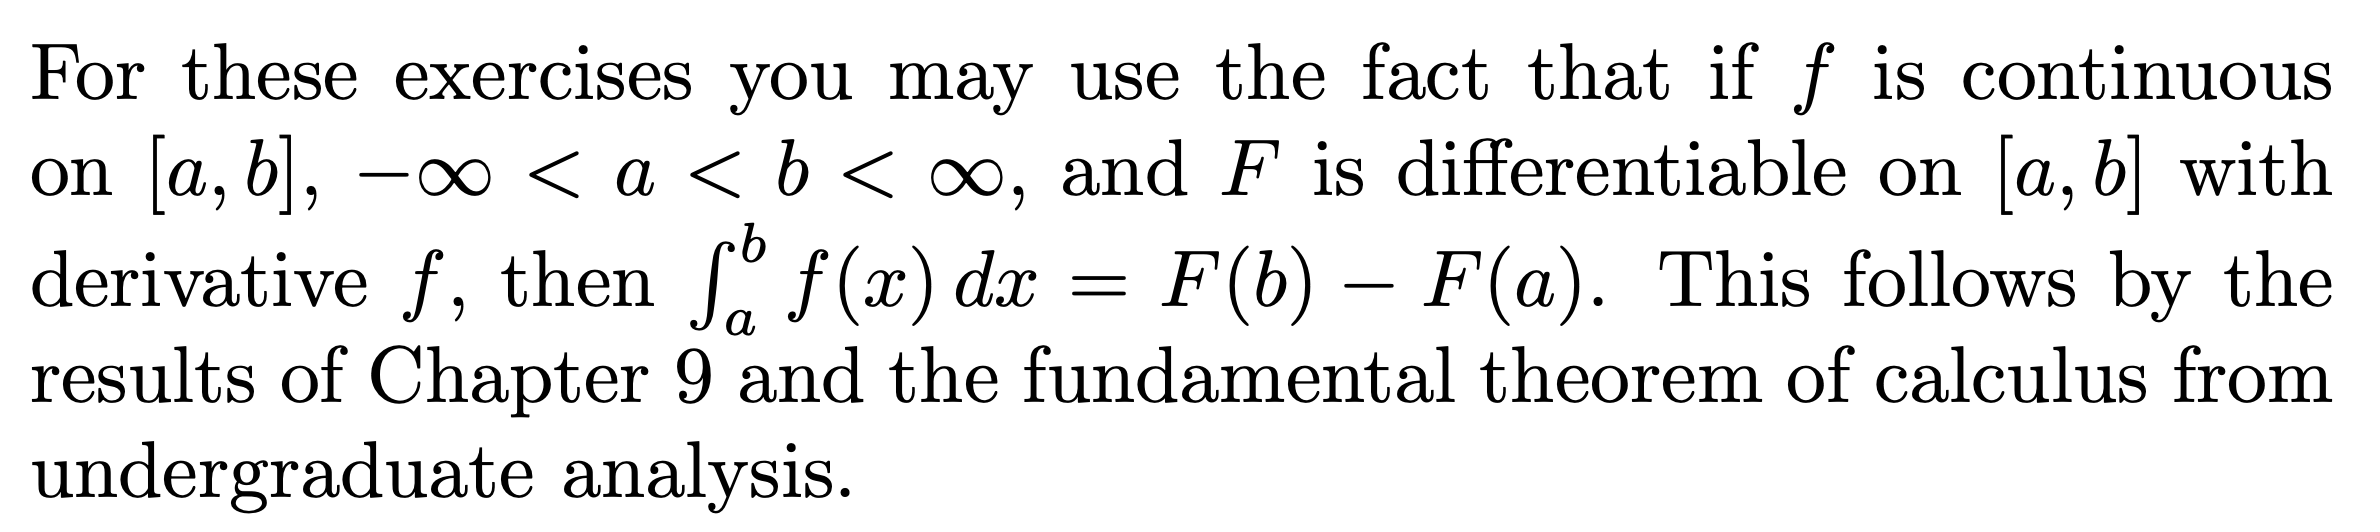
\includegraphics[width=400pt]{img/analysis--berkeley-202a-hw08-518d.png}
\end{mdframed}

\begin{mdframed}
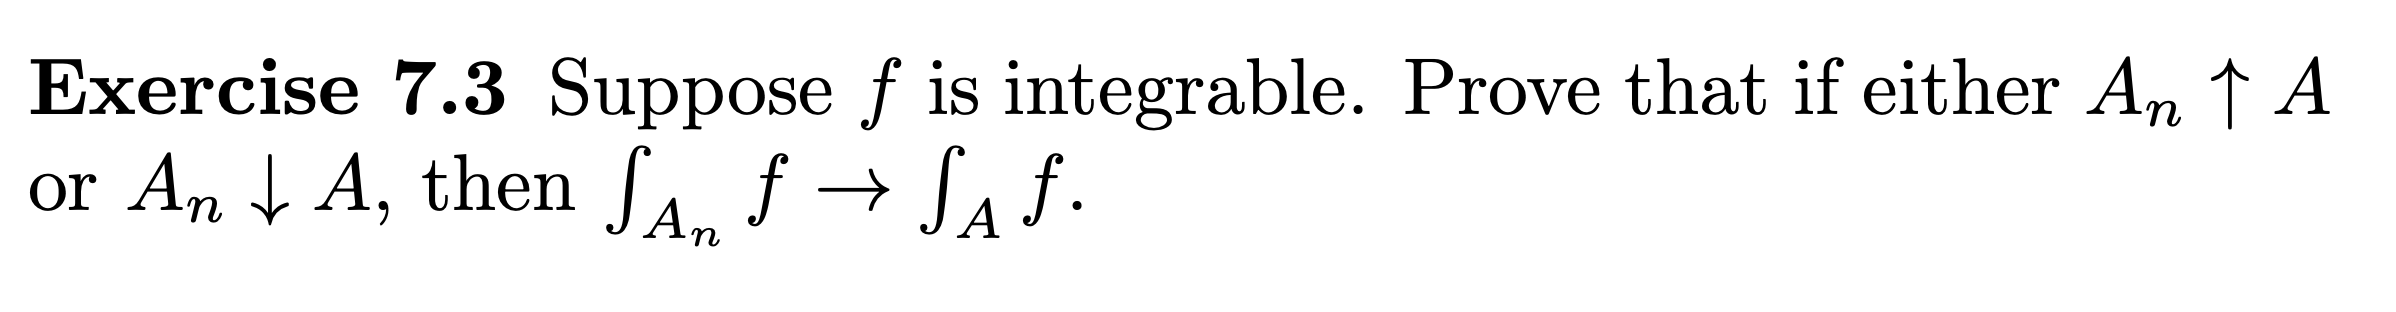
\includegraphics[width=400pt]{img/analysis--berkeley-202a-hw08-2798.png}
\end{mdframed}

\begin{proof}
  The required result is equivalent to
  \begin{align*}
    \limn \int f \ind_{A_n} = \int f \ind_A.
  \end{align*}

  Suppose first that $A_n \uparrow A$.

  Note that
  \begin{align*}
    \limn f\ind_{A_n} = f\limn\ind_{A_n} = f\ind_A,
  \end{align*}
  and furthermore that $|f\ind_{A_n}| \leq f$ for all $n$ and $f$ is integrable. Therefore by the dominated
  convergence theorem we have
  \begin{align*}
    \limn \int f \ind_{A_n} = \int f \ind_A,
  \end{align*}
  as required.

  Next suppose that $A_n \downarrow A$. Thus $A_n \supseteq A$ for all $n$, and $A_n^c \uparrow A^c$. In
  parallel with the previous argument we have
  \begin{align*}
    \limn f\ind_{A_n^c} = f\limn\ind_{A_n^c} = f\ind_{A^c},
  \end{align*}
  and furthermore $|f\ind_{A_n^c}| \leq f$ for all $n$ and $f$ is integrable.  Therefore by the dominated
  convergence theorem we have
  \begin{align*}
    \limn \int f \ind_{A_n^c} = \int f \ind_{A^c}.
  \end{align*}
  This can be written in terms of integrals over the original (non-complemented) sets as
  \begin{align*}
    \limn \Bigg(\int f - \int f \ind_{A_n}\Bigg) = \int f - \int f \ind_{A},
  \end{align*}
  or equivalently
  \begin{align*}
    \int f - \limn \int f \ind_{A_n} = \int f - \int f \ind_{A}.
  \end{align*}
  Since $\int f < \infty$ we may subtract $\int f$ from both sides, and then multiply by $-1$, yielding
  \begin{align*}
    \limn \int f \ind_{A_n} = \int f \ind_{A},
  \end{align*}
  as required.
\end{proof}

\begin{mdframed}
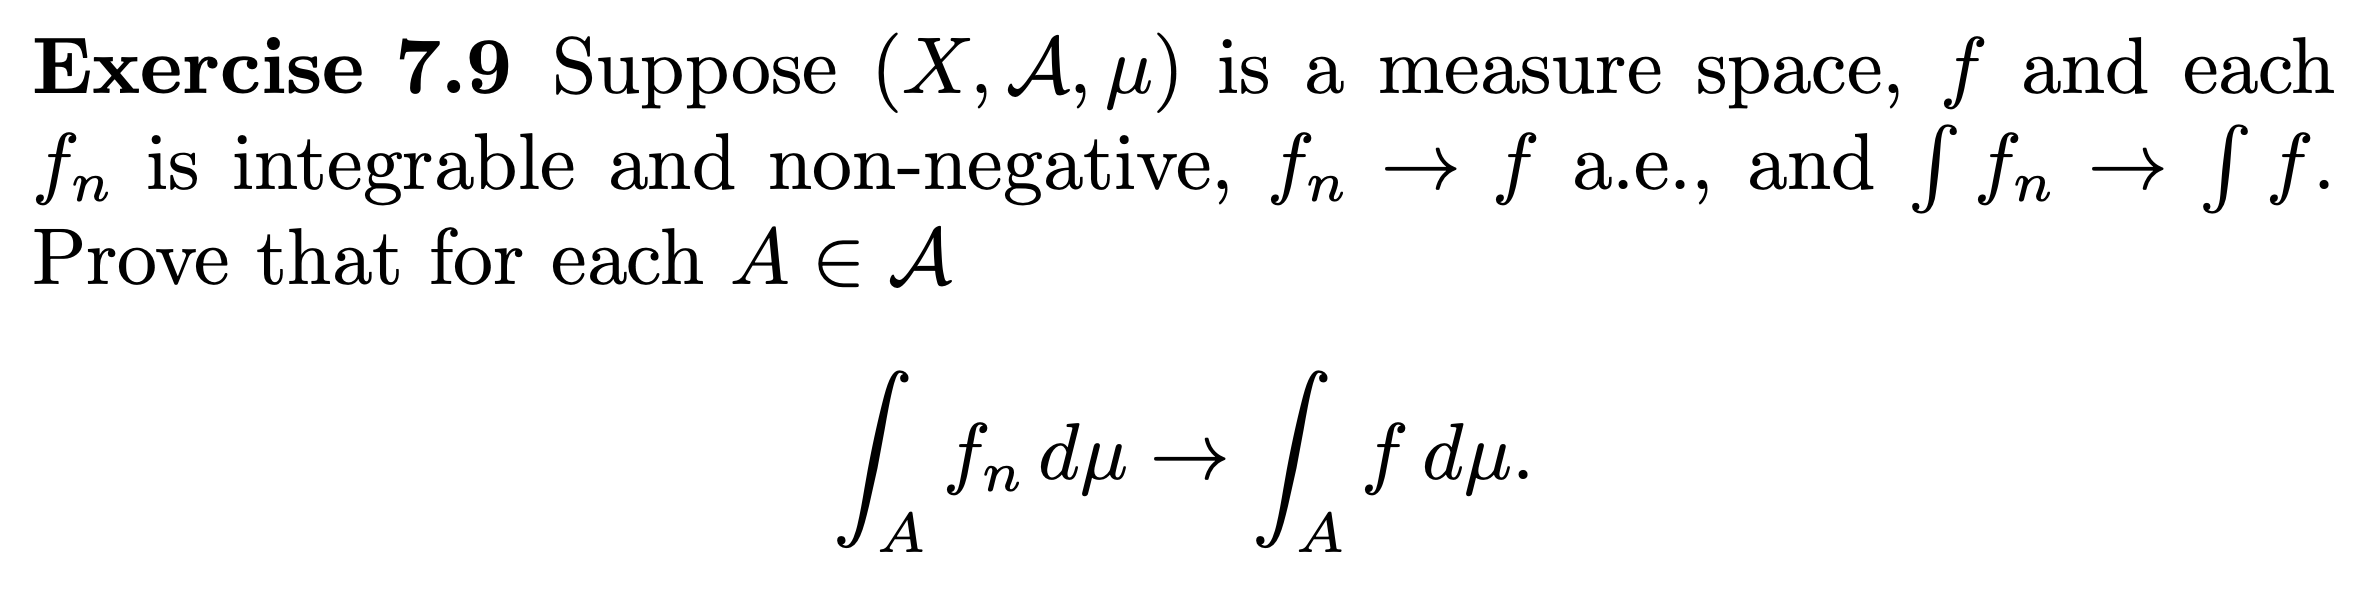
\includegraphics[width=400pt]{img/analysis--berkeley-202a-hw08-3203.png}
\end{mdframed}

\begin{proof}
  Note that $\int_A f_n = \int f_n\ind_A$ and that $f_n\ind_A \to f\ind_A$ a.e. Therefore by Fatou's lemma we have
  \begin{align*}
    \liminfn \int_A f_n \geq \int_A f.
  \end{align*}
  Now, we would like to show that
  \begin{align}
    \limsupn \int_A f_n \leq \int_A f.
  \end{align}
  since then we would have
  \begin{align*}
    \int_A f \leq \liminfn \int_A f_n \leq \limsupn \int_A f_n \leq \int_A f,
  \end{align*}
  which implies that
  \begin{align*}
    \limn \int_A f_n = \int f,
  \end{align*}
  as required.

  However, I'm not sure how to show (1).

  What have we made use of?
\begin{verbatim}
  |-------------------------+-------------|
  | non-negativity of f_n   | yes - Fatou |
  | convergence of f_n a.e. | yes         |
  | non-negativity of f     | no          |
  | integrability of f      | no          |
  | integrability of f_n    | no          |
  | convergence of int f_n  | no          |
\end{verbatim}
\end{proof}

\begin{remark*}
  We have that $\int_X f_n \to \int_X f$. What we must show is that this limit-of-integrals still holds when
  the integrals are restricted to $A \subset X$.

  In general, this is not true. For example, let $X = [0, 1]$ and let $f(x) = 0$. Now for odd $n$, let $f_n(x)$
  take the value $-1$ for $0 \leq x < 0.5$ and $+1$ for $0.5 \leq x \leq 1$, and for even $n$ let it take $+1$
  on the first interval and $-1$ on the second. Then $\int_X f_n = 0 = \int_X f$ for all $n$, so the
  hypothesis $\int_X f_n \to \int_X f$ does hold. But $\int_{[0, 0.5]} f_n$ is the
  sequence $-\frac{1}{2}, +\frac{1}{2}, -\frac{1}{2}, \ldots$ and thus has no limit.

  What we need to show is that the result does hold with the additional hypotheses.
\end{remark*}



\begin{mdframed}
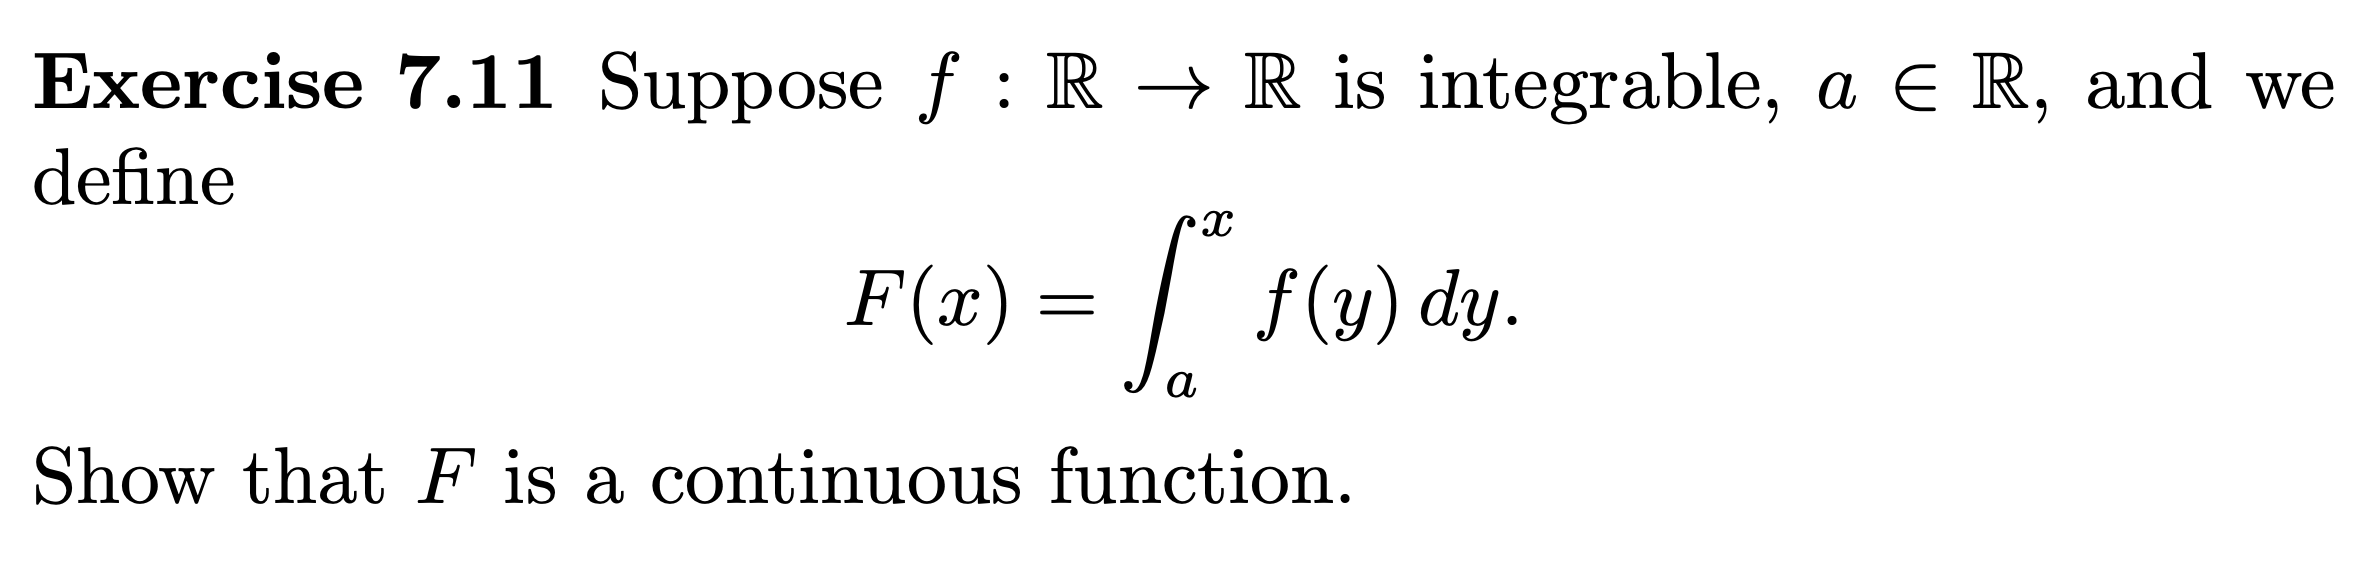
\includegraphics[width=400pt]{img/analysis--berkeley-202a-hw08-d0c0.png}
\end{mdframed}

\begin{intuition*}
  $F$ is an increasing function $\R \to \R$. To say that it is continuous is to say that a small extension to
  the interval being integrated over results in a small extension to the area. This implies that there is some
  limit to how much area is added by a small interval $[b, b + \delta]$.
\end{intuition*}

\begin{proof}
  Let $\eps > 0$ and let $b \in \R$.

  We must show that there exists $\delta > 0$ such that if $x \in \(b - \delta, b + \delta\)$
  then $F(x) \in \(F(b) - \eps, F(b) + \eps\)$.

  Note that $F$ is an increasing function, therefore it suffices to show that there exists $\delta$ such
  that $F(b - \delta) > F(b) - \eps$ and $F(b + \delta) < F(b) + \eps$.

  First we will show that there exists $\delta > 0$ such that $F(b + \delta) < F(b) + \eps$. Note that
  \begin{align*}
    F(b + \delta) := \int_{[a, b + \delta]} f = F(b) + \int_{[b, b + \delta]} f,
  \end{align*}
  therefore it suffices to show that there exists $\delta > 0$ such that $\int_{[b, b + \delta]} f < \eps$.
  This follows from HW7 Bass Ex. 6.4.

  Secondly we will show that there exists $\delta > 0$ such that $F(b - \delta) > F(b) - \eps$. Note that
  \begin{align*}
    F(b) = F(b - \delta) + \int_{[b - \delta, b]} f,
  \end{align*}
  hence
  \begin{align*}
    F(b - \delta) = F(b) - \int_{[b - \delta, b]} f,
  \end{align*}
  therefore it suffices to show that there exists $\delta > 0$ such that $\int_{[b - \delta, b]} f < \eps$.
  Again, this follows from HW7 Bass Ex. 6.4.
\end{proof}


\begin{mdframed}
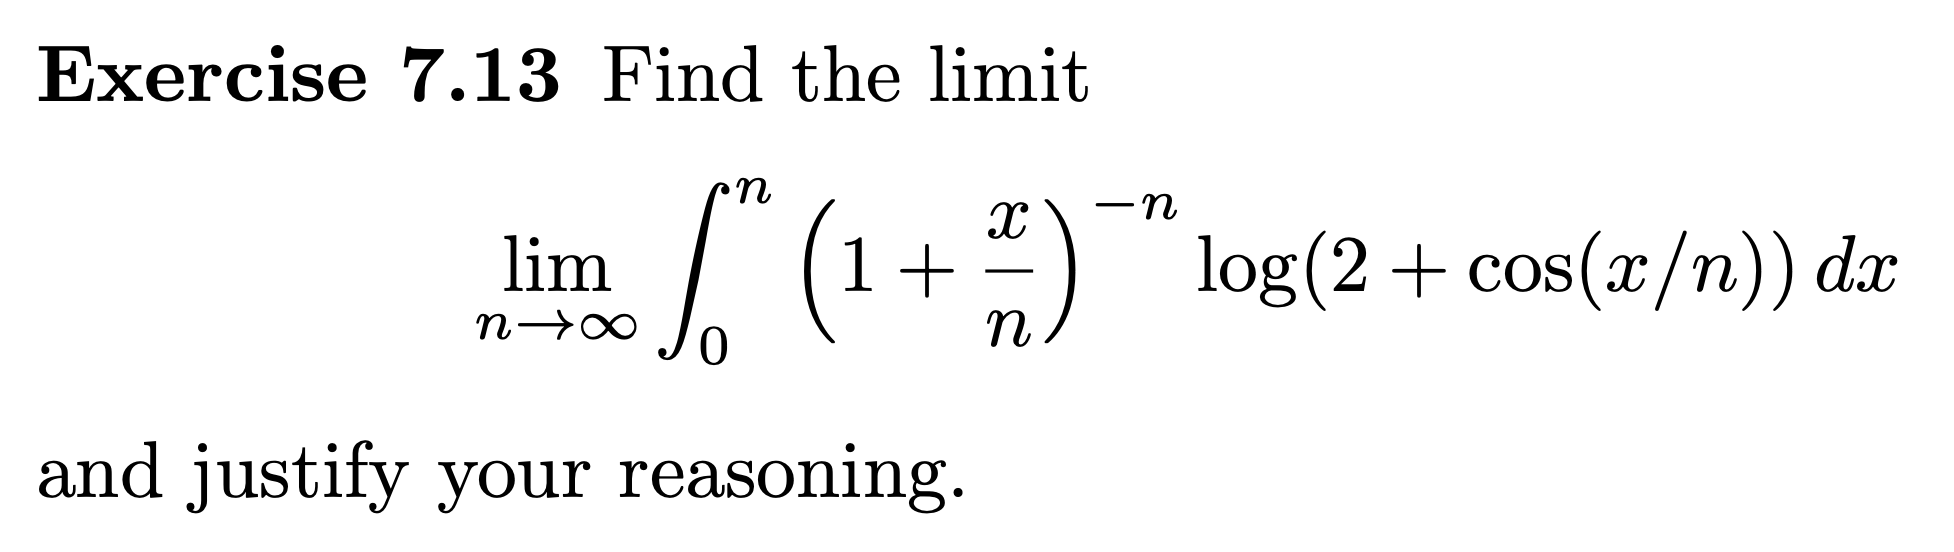
\includegraphics[width=400pt]{img/analysis--berkeley-202a-hw08-9931.png}
\end{mdframed}

\begin{proof}
  Let $f(n) = (1 + x/n)^{-n} \log(2 + \cos(x/n))$.

  Note that $2 + \cos(x/n) \geq 1$ and therefore that $f_n \geq 0$ for all $n$.

  Note also that $(f_n)$ is an increasing sequence, since (\red{TODO})
  \begin{align*}
    \frac{f_{n}}{f_{n+1}}
    &= \frac{(1 + x/n    )^{-n    } \log(2 + \cos(x/n   ))}
            {(1 + x/(n+1))^{-(n+1)} \log(2 + \cos(x/(n+1)))}.
  \end{align*}
  Therefore by the monotone convergence theorem we have
  \begin{align*}
    \limn \int_0^n f_n = \int_0^n \limn f_n.
  \end{align*}
  We can now compute the limit:
  \begin{align*}
    \limn (1 + x/n)^{-n} \log(2 + \cos(x/n))
    &= \log
  \end{align*}

\end{proof}

\begin{mdframed}
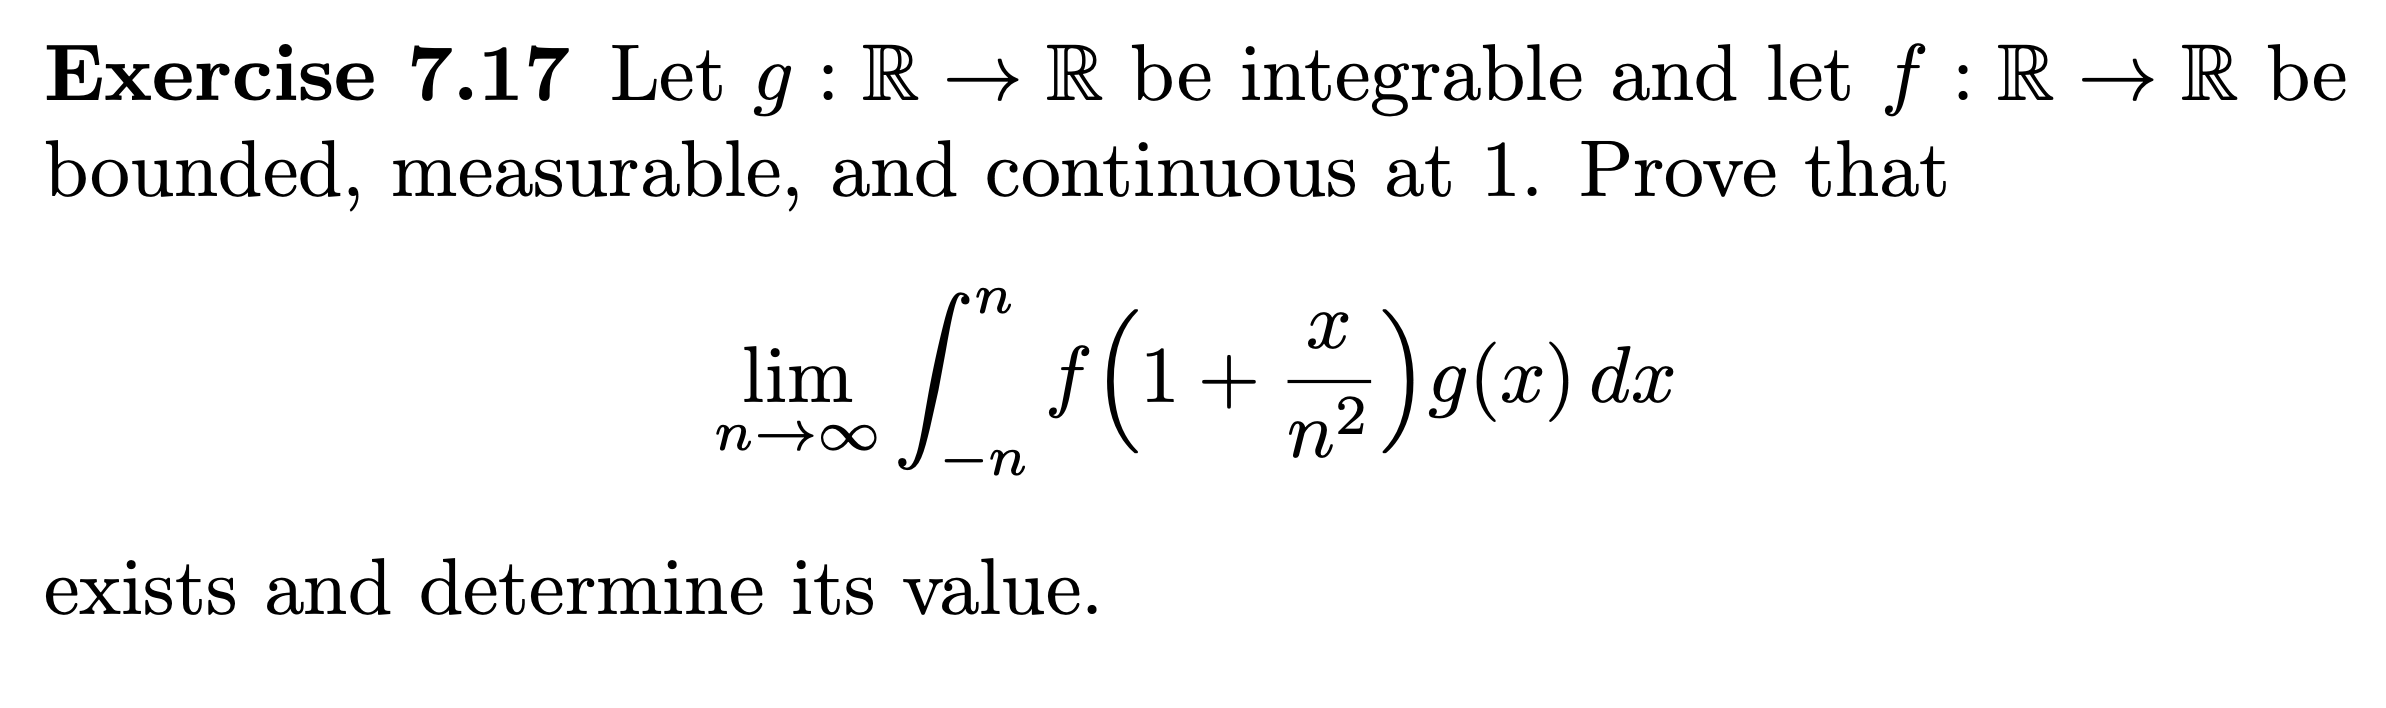
\includegraphics[width=400pt]{img/analysis--berkeley-202a-hw08-6e60.png}
\end{mdframed}


\begin{mdframed}
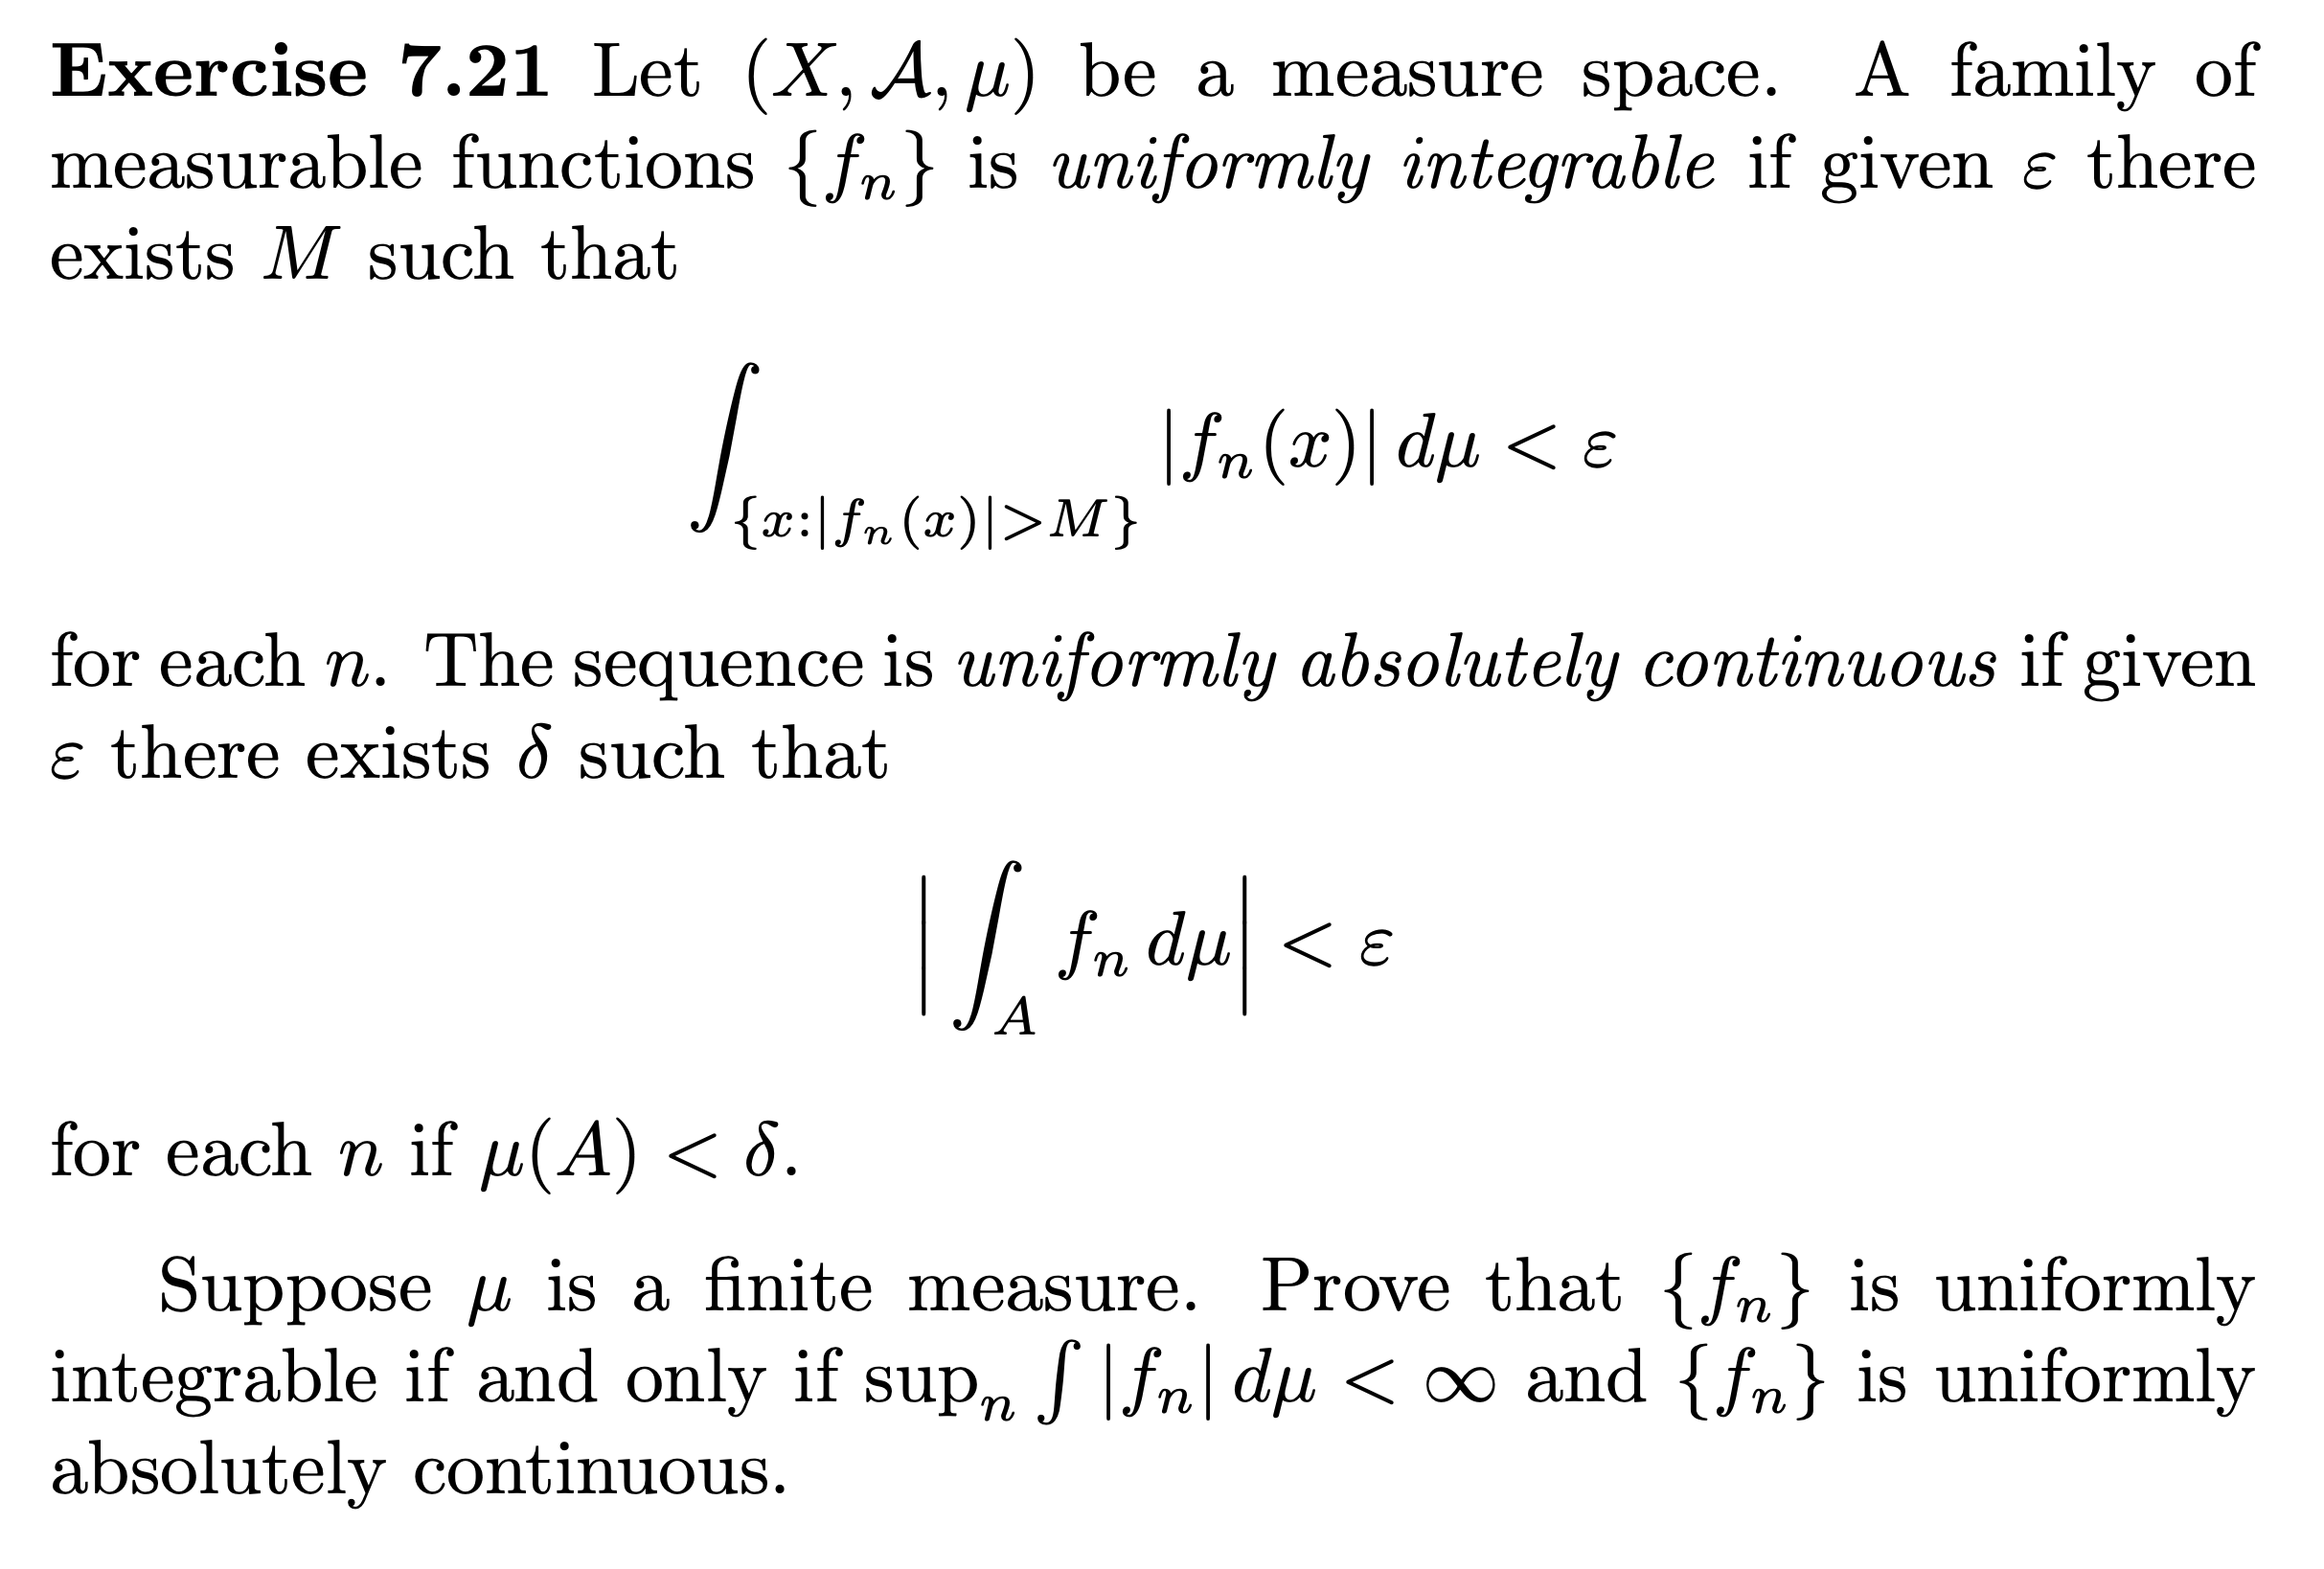
\includegraphics[width=400pt]{img/analysis--berkeley-202a-hw08-337f.png}
\end{mdframed}